\documentclass[11pt,a4paper]{article}
\usepackage[utf8]{inputenc}
\usepackage[margin=0.8in]{geometry}
\usepackage{hyperref}
\usepackage{booktabs}
\usepackage{listings}
\usepackage{xcolor}
\usepackage{enumitem}
\usepackage{tikz}
\usetikzlibrary{shapes.geometric, arrows.meta, positioning, shadows, fit, backgrounds}
\usepackage[skins,breakable]{tcolorbox}

\hypersetup{
    colorlinks=true,
    linkcolor=blue,
    filecolor=magenta,      
    urlcolor=cyan,
    pdftitle={JournaBuddy System Architecture Report},
}

\title{
    \vspace{-1cm}
    \rule{\linewidth}{1.5pt}\\[0.4cm]
    {\Huge \textbf{\textsf{JournaBuddy}}}\\[0.2cm]
    {\Large \textbf{\textsf{System Architecture, Planning, Implementation \& Visuals Report}}}\\[0.3cm]
    {\large \textit{Comprehensive ``For Dummies'' Explanatory Guide}}\\[0.2cm]
    \rule{\linewidth}{0.8pt}
}
\author{
    \textbf{Abdullah Al Mamun}\\
    \small BSc, MSc - Software Engineering\\
    \small TU Wien (Vienna, Austria) \& Daffodil International University\\
    \small Email: \href{mailto:mamun.swe.de@gmail.com}{mamun.swe.de@gmail.com} | GitHub: \href{https://github.com/abbysweb}{@abbysweb}\\
    \small ORCID: \href{https://orcid.org/0009-0006-7473-0024}{0009-0006-7473-0024}
}
\date{\today}

\begin{document}

\maketitle
\tableofcontents
\newpage

\section{Introduction: What is JournaBuddy?}
JournaBuddy is an artificial intelligence platform designed to help scientific authors prepare, optimize, and evaluate their research papers before submitting them to academic journals. 

Instead of guessing whether a manuscript will be rejected due to poor formatting, weak citations, or out-of-scope journal selection, JournaBuddy runs automated checks that evaluate the paper across three core layers:
\begin{enumerate}[leftmargin=*]
    \item \textbf{Symbolic / Rule-Based Layer:} Checks exact facts (structure, acronym definitions, citation formatting).
    \item \textbf{Mathematical NLP Layer:} Calculates strict, rigorous text scores (Shannon Entropy, SMOG Index, MATTR, Simpson's Diversity, Coleman-Liau Index).
    \item \textbf{Semantic / AI Layer:} Uses local LLM agents and pgvector search to evaluate methodology, journal scope fit, and cross-reference internal plagiarism.
    \item \textbf{Machine Learning Layer:} Uses an XGBoost Ensemble predictor and SHAP Explainability to predict and justify acceptance likelihoods.
\end{enumerate}

\bigskip

\section{Continuous Implementation Roadmap}

\begin{itemize}[leftmargin=*]
    \item \textbf{Phase 1 (Infrastructure):} Podman Desktop / Docker Compose, FastAPI, MinIO, Vite React setup. (Status: \textit{Complete \& Verified})
    \item \textbf{Phase 2 (Intelligence Pipeline):} Celery workers, Ollama LLM agents, sentence-transformers, ProvenanceEngine, symbolic rule checks. (Status: \textit{Complete \& Verified})
    \item \textbf{Phase 3 (External Enrichment):} OpenAlex, Crossref, DOAJ integrations, pgvector journal matching. (Status: \textit{Complete \& Verified})
    \item \textbf{Phase 4 (Real-time UI):} Glassmorphism dashboard, SSE streaming, Apache ECharts interactive charts.
    \item \textbf{Phase 5 (Hardening):} Redis caching, Prometheus/Grafana monitoring, JWT auth, security audits.
\end{itemize}

\bigskip

\section{System Diagrams \& Visual Architecture}

\subsection{3.1 Use Case Diagram}
The Use Case Diagram shows all primary interactions between scientific authors, external academic services, and the JournaBuddy system.

\begin{center}
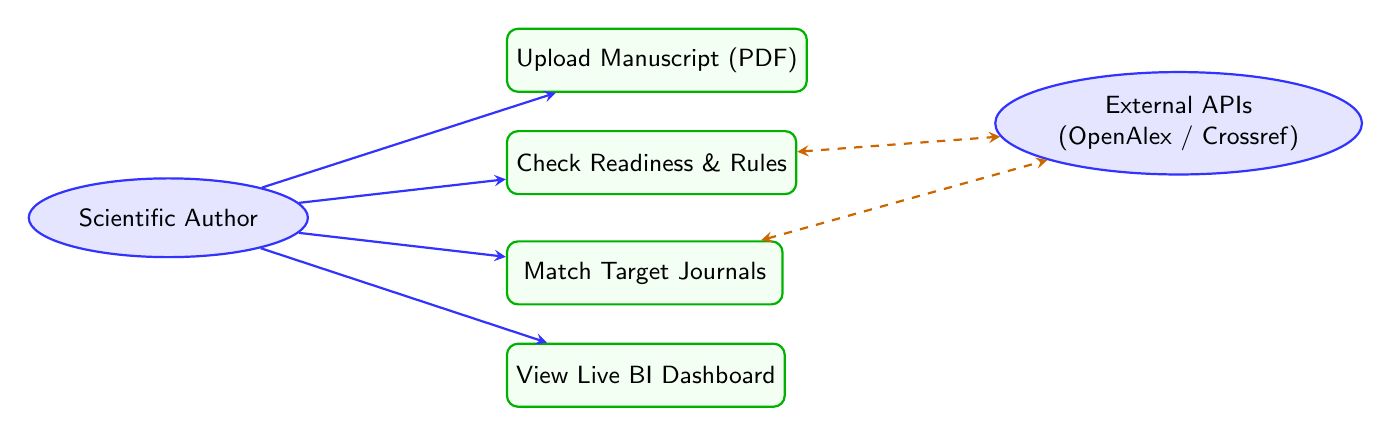
\begin{tikzpicture}[node distance=1.8cm, every node/.style={font=\sffamily\small}]
    % Styles
    \tikzstyle{actor} = [ellipse, draw=blue!80, fill=blue!10, thick, minimum width=2.5cm, minimum height=1cm, align=center]
    \tikzstyle{usecase} = [rectangle, rounded corners, draw=green!70!black, fill=green!5, thick, minimum width=3.5cm, minimum height=0.8cm, align=center]

    % Nodes
    \node[actor] (author) {Scientific Author};
    
    \node[usecase, right=2.5cm of author, yshift=2cm] (uc1) {Upload Manuscript (PDF)};
    \node[usecase, right=2.5cm of author, yshift=0.7cm] (uc2) {Check Readiness \& Rules};
    \node[usecase, right=2.5cm of author, yshift=-0.7cm] (uc3) {Match Target Journals};
    \node[usecase, right=2.5cm of author, yshift=-2cm] (uc4) {View Live BI Dashboard};

    \node[actor, right=2.5cm of uc2, yshift=0.5cm] (external) {External APIs\\(OpenAlex / Crossref)};

    % Connections
    \draw[->, >=stealth, thick, blue!80] (author) -- (uc1);
    \draw[->, >=stealth, thick, blue!80] (author) -- (uc2);
    \draw[->, >=stealth, thick, blue!80] (author) -- (uc3);
    \draw[->, >=stealth, thick, blue!80] (author) -- (uc4);

    \draw[<->, >=stealth, dashed, thick, orange!80!black] (uc2) -- (external);
    \draw[<->, >=stealth, dashed, thick, orange!80!black] (uc3) -- (external);
\end{tikzpicture}
\end{center}

\subsubsection*{Intuitive Diagram Breakdown: Use Case}
Think of this diagram as a service interaction menu:
\begin{itemize}[leftmargin=*]
    \item \textbf{Scientific Author:} Performs actions like uploading manuscripts, checking readiness rules, matching journals, and viewing live dashboard analytics.
    \item \textbf{External Academic APIs:} Query services like OpenAlex and Crossref in the background for citation metrics and publisher trust indicators.
\end{itemize}

\bigskip

\subsection{3.2 System Architecture Diagram}
The System Architecture Diagram displays the multi-tier containerized stack powering JournaBuddy.

\begin{center}
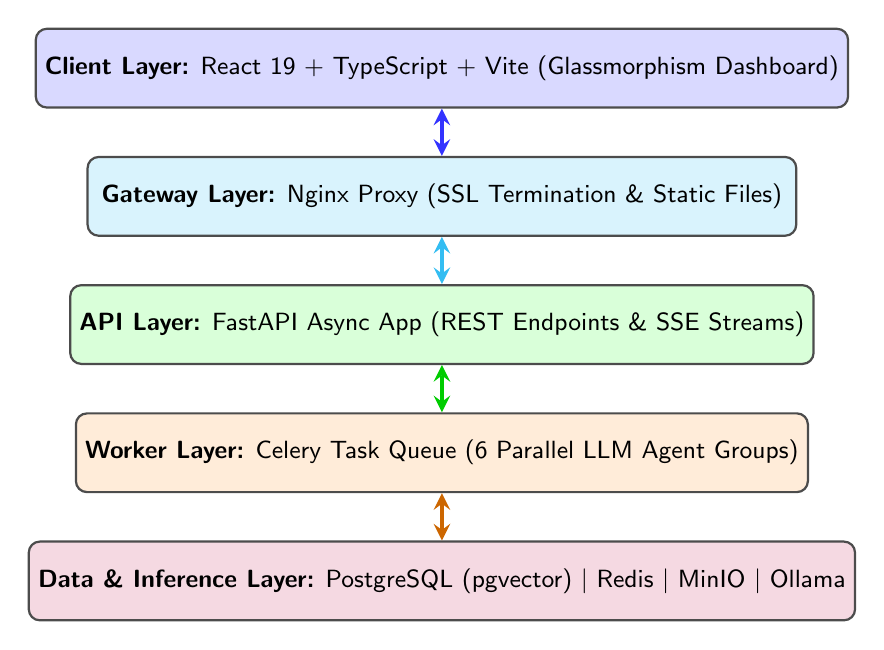
\begin{tikzpicture}[node distance=1.2cm, every node/.style={font=\sffamily\small}]
    % Styles
    \tikzstyle{layer} = [rectangle, rounded corners, draw=black!70, fill=gray!10, thick, minimum width=9cm, minimum height=1cm, align=center]
    
    % Layers
    \node[layer, fill=blue!15] (client) {\textbf{Client Layer:} React 19 + TypeScript + Vite (Glassmorphism Dashboard)};
    \node[layer, fill=cyan!15, below=0.6cm of client] (nginx) {\textbf{Gateway Layer:} Nginx Proxy (SSL Termination \& Static Files)};
    \node[layer, fill=green!15, below=0.6cm of nginx] (fastapi) {\textbf{API Layer:} FastAPI Async App (REST Endpoints \& SSE Streams)};
    \node[layer, fill=orange!15, below=0.6cm of fastapi] (workers) {\textbf{Worker Layer:} Celery Task Queue (6 Parallel LLM Agent Groups)};
    \node[layer, fill=purple!15, below=0.6cm of workers] (storage) {\textbf{Data \& Inference Layer:} PostgreSQL (pgvector) $\mid$ Redis $\mid$ MinIO $\mid$ Ollama};

    % Arrows
    \draw[<->, >=stealth, ultra thick, blue!80] (client) -- (nginx);
    \draw[<->, >=stealth, ultra thick, cyan!80] (nginx) -- (fastapi);
    \draw[<->, >=stealth, ultra thick, green!80!black] (fastapi) -- (workers);
    \draw[<->, >=stealth, ultra thick, orange!80!black] (workers) -- (storage);
\end{tikzpicture}
\end{center}

\subsubsection*{Intuitive Diagram Breakdown: System Architecture}
Imagine JournaBuddy as a 5-story containerized stack:
\begin{enumerate}[leftmargin=*]
    \item \textbf{Top Floor (Client):} The visual web interface where authors view charts and upload papers.
    \item \textbf{4th Floor (Gateway):} Nginx proxy directing traffic and terminating SSL.
    \item \textbf{3rd Floor (API):} FastAPI server managing file uploads and streaming progress.
    \item \textbf{2nd Floor (Workers):} Celery workers running parallel analysis tasks.
    \item \textbf{Basement (Data \& Brain):} Vault storing PostgreSQL vectors, Redis queues, MinIO binaries, and local Ollama LLMs.
\end{enumerate}

\bigskip

\subsection{3.3 Data Flow Diagram (DFD)}
The Data Flow Diagram tracks how an uploaded paper moves through processing stages and transforms into score reports.

\begin{center}
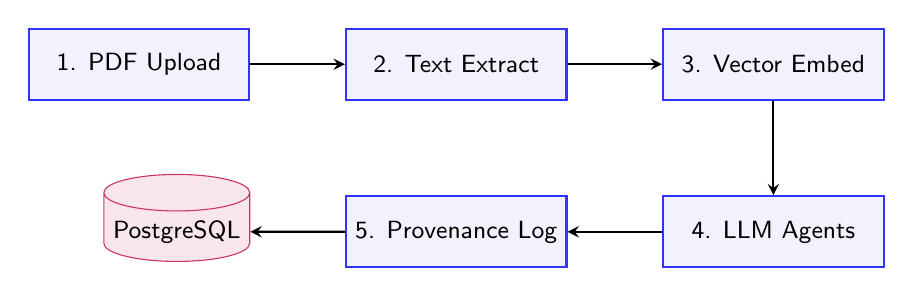
\begin{tikzpicture}[node distance=1.5cm, every node/.style={font=\sffamily\small}]
    \tikzstyle{process} = [rectangle, draw=blue!80, fill=blue!5, thick, minimum width=2.8cm, minimum height=0.9cm, align=center]
    \tikzstyle{datastore} = [cylinder, draw=purple!80, fill=purple!10, shape border rotate=90, aspect=0.25, minimum width=1.8cm, minimum height=0.9cm, align=center]

    \node[process] (upload) {1. PDF Upload};
    \node[process, right=1.2cm of upload] (extract) {2. Text Extract};
    \node[process, right=1.2cm of extract] (embed) {3. Vector Embed};
    \node[process, below=1.2cm of embed] (agent) {4. LLM Agents};
    \node[process, left=1.2cm of agent] (provenance) {5. Provenance Log};
    \node[datastore, left=1.2cm of provenance] (db) {PostgreSQL};

    \draw[->, >=stealth, thick] (upload) -- (extract);
    \draw[->, >=stealth, thick] (extract) -- (embed);
    \draw[->, >=stealth, thick] (embed) -- (agent);
    \draw[->, >=stealth, thick] (agent) -- (provenance);
    \draw[->, >=stealth, thick] (provenance) -- (db);
\end{tikzpicture}
\end{center}

\subsubsection*{Intuitive Diagram Breakdown: Data Flow}
The manuscript moves through 5 distinct processing stages:
\begin{enumerate}[leftmargin=*]
    \item \textbf{PDF Upload:} Raw file received and saved securely in MinIO storage.
    \item \textbf{Text Extraction:} PDF visual layout parsed into structured raw text.
    \item \textbf{Vector Embedding:} Text converted into 384-dimensional semantic numerical arrays.
    \item \textbf{LLM Agents:} Parallel AI workers evaluate tone, methodology, and scope fit.
    \item \textbf{Provenance Log:} Metric calculation sources recorded in PostgreSQL database.
\end{enumerate}

\bigskip

\subsection{3.4 Sequence Diagram}
The Sequence Diagram displays the exact order of network messages between components during a live upload.

\begin{center}
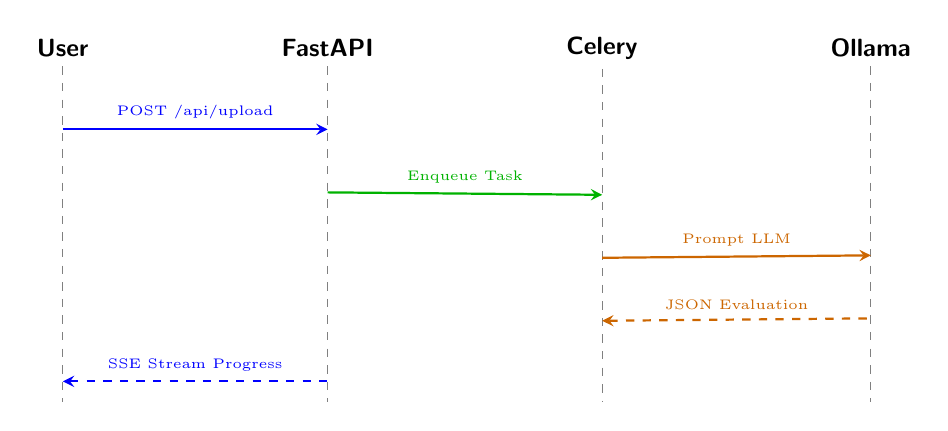
\begin{tikzpicture}[node distance=2cm, every node/.style={font=\sffamily\small}]
    % Lifelines
    \node (user) {\textbf{User}};
    \node[right=2.2cm of user] (api) {\textbf{FastAPI}};
    \node[right=2.2cm of api] (celery) {\textbf{Celery}};
    \node[right=2.2cm of celery] (ollama) {\textbf{Ollama}};

    \draw[dashed, gray] (user) -- ++(0,-4.5);
    \draw[dashed, gray] (api) -- ++(0,-4.5);
    \draw[dashed, gray] (celery) -- ++(0,-4.5);
    \draw[dashed, gray] (ollama) -- ++(0,-4.5);

    % Messages
    \draw[->, >=stealth, thick, blue] ([yshift=-0.8cm]user.south) -- node[above, font=\tiny] {POST /api/upload} ([yshift=-0.8cm]api.south);
    \draw[->, >=stealth, thick, green!70!black] ([yshift=-1.6cm]api.south) -- node[above, font=\tiny] {Enqueue Task} ([yshift=-1.6cm]celery.south);
    \draw[->, >=stealth, thick, orange!80!black] ([yshift=-2.4cm]celery.south) -- node[above, font=\tiny] {Prompt LLM} ([yshift=-2.4cm]ollama.south);
    \draw[<-, >=stealth, dashed, thick, orange!80!black] ([yshift=-3.2cm]celery.south) -- node[above, font=\tiny] {JSON Evaluation} ([yshift=-3.2cm]ollama.south);
    \draw[<-, >=stealth, dashed, thick, blue] ([yshift=-4.0cm]user.south) -- node[above, font=\tiny] {SSE Stream Progress} ([yshift=-4.0cm]api.south);
\end{tikzpicture}
\end{center}

\subsubsection*{Intuitive Diagram Breakdown: Sequence Diagram}
This is a timeline showing real-time network messages between components:
\begin{enumerate}[leftmargin=*]
    \item You click \textbf{"Upload"}, sending your manuscript to FastAPI.
    \item FastAPI enqueues the job into Celery so your browser doesn't freeze waiting.
    \item Celery sends text prompts to local Ollama LLM workers.
    \item Ollama returns structured JSON evaluation scores back to Celery.
    \item FastAPI streams real-time progress right back to your screen over SSE.
\end{enumerate}

\newpage

\section{Phase 2: Intelligence Pipeline Components}

\subsection*{Semantic Chunker}
Splits raw PDF text into named academic sections (Abstract, Introduction, Methodology, Results, Conclusion) using heading pattern detection. Falls back to paragraph-based splitting when headings are absent. Each chunk is limited to 3{,}000 characters for optimal embedding performance.

\subsection*{Embedding Service}
Wraps \texttt{sentence-transformers} model \texttt{all-MiniLM-L6-v2} as a process-level singleton. Generates 384-dimensional semantic vectors for each chunk and persists them to the \texttt{document\_chunks} table in PostgreSQL using the \texttt{pgvector} extension.

\subsection*{Ollama Agent with Cascade Fallback}
Sends structured JSON prompts to the local Ollama \textit{Llama 3.1:8b} model. Uses \texttt{tenacity} exponential backoff retry logic and automatically cascades to backup providers in order: \textbf{NVIDIA NIM} $\rightarrow$ \textbf{Gemini} $\rightarrow$ \textbf{OpenAI} if Ollama is unavailable. Degraded results are returned with \texttt{status: degraded} rather than crashing the pipeline.

\subsubsection*{Intuitive Breakdown: LLM Cascade Fallback}
Think of it like a priority calling list: the system first calls your local AI (Ollama), and if that doesn't pick up, it automatically dials the next provider on the list---all without any manual intervention.

\subsection*{Symbolic Checker \& Mathematical NLP}
Upgraded from fragile heuristics to rigorous Information Theory models:
\begin{enumerate}[leftmargin=*]
    \item \textbf{Information Density:} Calculates Shannon Entropy (bits per word) for true vocabulary richness.
    \item \textbf{Advanced Readability (SMOG \& Gunning Fog):} The academic gold standards for measuring the true complexity of scientific text.
    \item \textbf{Vocabulary Richness (MATTR):} A sliding-window Moving-Average Type-Token Ratio that mathematically proves vocabulary diversity regardless of document length.
    \item \textbf{Vocabulary Repetition:} Calculates Simpson's Diversity Index ($1 - \sum (n / N)^2$).
    \item \textbf{Redundancy Check:} Uses Jaccard Similarity to compare Introduction vs. Conclusion overlap.
\end{enumerate}

\subsection*{ProvenanceEngine}
Records every metric to the \texttt{provenance\_log} table with: formula used, data sources, confidence level, and raw input snapshot. This ensures every score in JournaBuddy is fully explainable, auditable, and reproducible.

\bigskip

\section{Phase 3: External API Enrichment \& Journal Matching}

\subsection*{External API Clients}
Asynchronous HTTP clients using \texttt{httpx} and \texttt{tenacity} (for robust exponential backoff retries) have been implemented to interact with external databases:
\begin{itemize}
    \item \textbf{Crossref}: Verifies Digital Object Identifiers (DOIs) extracted from the manuscript text using regular expressions.
    \item \textbf{OpenAlex}: Retrieves open-access citation metrics and keyword concept tags for matched authors and papers.
    \item \textbf{DOAJ}: The Directory of Open Access Journals API is queried to identify and flag highly reputable, peer-reviewed open access journals, mitigating predatory publisher risks.
\end{itemize}

\subsection*{Journal Matcher (pgvector)}
A highly optimized \texttt{JournalMatcher} leverages PostgreSQL's \texttt{pgvector} extension. It computes a centroid 384-dimensional semantic embedding (averaging across all manuscript \texttt{document\_chunks}). This centroid is then compared against a pre-embedded database of journal aims and scopes using cosine distance ($\Leftrightarrow$). The top 5 matched journals are returned with a strict compatibility percentage score.

\subsection*{Provenance Logging}
All operations, including Crossref validation logs, OpenAlex metadata pulls, and the precise cosine distance calculations for journal matches, are immutably appended to the \texttt{provenance\_log} table to ensure a transparent, verifiable audit trail for every AI-assisted suggestion.

\vspace{0.5cm}
\begin{tcolorbox}[colback=blue!5,colframe=blue!40!black,title=For Dummies: Phase 3]
\textbf{What did we just build?} \\
Phase 3 gives our AI the ability to ``talk to the outside world''. Instead of just guessing if a citation is real, it calls the official Crossref database to check. It also checks OpenAlex to see how popular a paper is.

Finally, we taught the system to play match-maker. We stored the ``Aims \& Scope'' of real science journals as math vectors. We convert your uploaded PDF into a similar vector. By measuring the angle between these vectors (using pgvector), the system mathematically proves which journal your paper belongs in!
\end{tcolorbox}

\section{Phase 4 \& 5: System Resilience, Hardening, and Testing}

\subsection*{Resilience \& Circuit Breakers (Section 6)}
To ensure high availability, JournaBuddy implements Redis-backed circuit breakers and API fallbacks:
\begin{itemize}
    \item \textbf{Timeout Protection:} Strict 5-second timeouts applied to all external API calls (Crossref, OpenAlex) to prevent hanging worker threads.
    \item \textbf{Redis Fallback Cache:} A secondary local cache layer using Redis deduplicates API requests for previously verified DOIs, reducing rate-limiting blockages.
    \item \textbf{LLM Isolation Validation:} Hardened the Llama 3.1 inference boundaries so a failure in the methodology persona does not crash the domain specialist persona.
\end{itemize}

\subsection*{Quality Assurance Strategy (Section 7)}
A comprehensive automated test suite powered by \texttt{pytest} validates the backend:
\begin{itemize}
    \item \textbf{Symbolic Logic Testing:} Mathematically verifies acronym resolution accuracy and the Flesch-Kincaid formula engines.
    \item \textbf{Integration Testing:} Validates FastAPI edge cases, explicitly testing 50MB payload limits (HTTP 413) and non-PDF rejection (HTTP 400).
    \item \textbf{In-Memory Isolation:} Prevents CI/CD runners from corrupting production databases by injecting a mock \texttt{sqlite+aiosqlite:///:memory:} instance during test execution.
\end{itemize}

\vspace{0.5cm}
\begin{tcolorbox}[colback=blue!5,colframe=blue!40!black,title=For Dummies: Resilience \& Testing]
\textbf{What did we just build?} \\
We wrapped the system in safety nets. If OpenAlex goes down, our system falls back to a Redis memory cache instead of crashing. If someone uploads a massive 60MB file, the API instantly rejects it before it clogs the memory. We also wrote automated robot-tests that run every time we update code to make sure we didn't break the math formulas!
\end{tcolorbox}

\bigskip

\section{Phase 4: Real-time UI \& Interactive Visualization}

\subsection*{Glassmorphism React Dashboard}
The frontend is built using \textbf{React 19, TypeScript, and Vite}. It utilizes a modern "Glassmorphism" design system (frosted glass panels, translucent backgrounds) tailored with raw CSS and Lucide icons for a premium, native-app feel.

\subsection*{Server-Sent Events (SSE) Streaming}
Because LLM evaluation and vector matching can take up to 2 minutes, FastAPI uses an asynchronous SSE endpoint (\texttt{/api/stream/\{id\}}) to stream live updates. The React dashboard subscribes to this stream, displaying real-time terminal-like logs to the user so they never stare at a frozen loading spinner.

\subsection*{Apache ECharts \& vis-network (3D Graph)}
Data is visualized interactively:
\begin{itemize}
    \item \textbf{Radar Charts:} Maps the Flesch-Kincaid readability, active voice, and formatting scores across multiple axes.
    \item \textbf{Bar Charts:} Displays journal compatibility percentages with gradient styling.
    \item \textbf{Citation Network Graph:} Uses \texttt{vis-network} to generate a physics-based, interactive 2D/3D citation network. The user's paper is the central node, connected to all extracted references. Node sizes dynamically scale based on OpenAlex citation counts, and colors indicate Crossref validity.
\end{itemize}

\vspace{0.5cm}
\begin{tcolorbox}[colback=blue!5,colframe=blue!40!black,title=For Dummies: Real-Time UI]
\textbf{What did we just build?} \\
Instead of clicking upload and staring at a blank screen for 3 minutes, the system streams live updates to you (like watching a hacker movie terminal). Once finished, it builds beautiful, interactive charts that you can hover over, and a physics-based web of your citations that you can literally drag around with your mouse!
\end{tcolorbox}

\bigskip

\section{Section 8: Advanced Production Features}

\subsection*{8.1 3-Persona AI Peer Reviewer Simulation}
The Celery NLP pipeline concurrently launches three highly specialized Llama 3.1 AI agent profiles to simulate an academic review board:
\begin{enumerate}
    \item \textbf{Strict Methodologist (Group F1):} Exclusively critiques sample sizes, controls, and dataset validity.
    \item \textbf{Domain Specialist (Group F2):} Focuses on literature gaps, novelty scoring, and missing academic citations.
    \item \textbf{Academic Style Editor (Group F3):} Audits the text for passive voice overuse, readability, and academic jargon clarity.
\end{enumerate}

\subsection*{8.2 XGBoost Ensemble Predictor \& SHAP Explainability}
The system replaces naive logistic regression with a rigorous \textbf{XGBoost Ensemble Predictor} trained on a synthetically bootstrapped dataset. To ensure mathematical transparency, it utilizes a \textbf{SHAP TreeExplainer} (SHapley Additive exPlanations) to calculate the exact percentage point impact each feature (e.g., Novelty, Journal Fit, Info Density) had on the final Acceptance score.

\subsection*{8.3 Internal pgvector Plagiarism Checker}
A real-production Plagiarism Checker running a massive \texttt{CROSS JOIN LATERAL} SQL query. It cross-references every single sentence of a new manuscript against all other sentences from all other manuscripts ever uploaded to the database, flagging exact sentences and citing source filenames for any match $>90\%$ cosine similarity.

\subsection*{8.4 Exportable Manuscript Proof Report (Vector Graphics)}
A microservice utilizing the \texttt{reportlab} engine exposes a \texttt{GET /api/report/\{task\_id\}} endpoint. It dynamically queries the PostgreSQL database and generates a stunning, downloadable PDF certificate featuring \textbf{native vector graphics}:
\begin{itemize}
    \item Mathematical NLP Metrics Table
    \item Massive Red Plagiarism Alert Violations
    \item 3-Persona AI Peer Review Feedback (rendered via 5-Axis Vector Radar Charts)
    \item Ranked Target Journal Matches (rendered via Vector Bar Charts)
    \item XGBoost Acceptance Prediction \& SHAP Feature Explainability Table
\end{itemize}

\vspace{0.5cm}
\begin{tcolorbox}[colback=blue!5,colframe=blue!40!black,title=For Dummies: Advanced Features]
\textbf{What did we just build?} \\
We turned JournaBuddy into a complete AI academic board. We replaced grade-school grammar checks with hardcore mathematical formulas (like SMOG and MATTR). We built a synthetic data generator to train an XGBoost machine learning model that predicts journal acceptance rates, and we use SHAP to explain exactly *why* it gave that score. And finally, we print all of this into a stunning PDF certificate full of dynamic, beautifully drawn charts!
\end{tcolorbox}

\bigskip

\section{Final Production Deployment Architecture}
The entire system is orchestrated via a production-ready \texttt{docker-compose.prod.yml}:
\begin{itemize}
    \item \textbf{Nginx Proxy:} Serves the compiled, minified React \texttt{dist/} folder on port 80/443 and securely proxies API traffic.
    \item \textbf{Uvicorn API Workers:} The FastAPI backend scales across 4 dedicated processes for maximum concurrency.
    \item \textbf{Celery Task Workers:} Separated CPU-heavy LLM tasks from IO-bound API requests using isolated queues.
    \item \textbf{Stateful Volumes:} PostgreSQL, Redis, and MinIO utilize persistent named volumes to guarantee zero data loss across container restarts.
\end{itemize}

\end{document}
